\section{Método: o simulador e sua validação}\label{sec:metodo}
% orçamento: 1.300 palavras

\subsection{Fundamentação física}\label{cap:fisica}

Este capítulo desenvolve a física que o simulador calcula. Partimos da lei da gravitação, escrevemos as equações de movimento de $N$ corpos e resolvemos o caso de dois corpos, que é o que dá as leis de Kepler e a linguagem dos elementos orbitais. As derivações seguem a linha de textos clássicos de mecânica e mecânica celeste \cite{symon1982,goldstein2002,murray1999,danby1988}. Algumas passagens mais longas estão no \autoref{ap:derivacoes}.

\subsubsection{Gravitação universal}

Dois corpos de massas $m_1$ e $m_2$, nas posições $\vr_1$ e $\vr_2$, atraem-se com força
\begin{equation}
  \vetor{F}_{12} = G\,\frac{m_1 m_2}{|\vr_2-\vr_1|^3}\,(\vr_2-\vr_1),
  \label{eq:newton}
\end{equation}
dirigida de um para o outro e proporcional ao inverso do quadrado da distância. Pela segunda lei de Newton, a aceleração do corpo 1 é $\va_1 = \vetor{F}_{12}/m_1$, e a massa $m_1$ se cancela: a aceleração que um corpo sofre não depende da própria massa, só da massa de quem o puxa.

\begin{paracomecar}
Uma pena e um martelo caem juntos na Lua, onde não há ar. Pela mesma razão, a Terra e um satélite artificial percorreriam a mesma órbita em torno do Sol se estivessem no mesmo lugar com a mesma velocidade.
\end{paracomecar}

\paragraph{Unidades e o parâmetro gravitacional}

Em mecânica celeste é mais conveniente trabalhar com o produto $GM$, o \emph{parâmetro gravitacional}, do que com $G$ e $M$ separados. O motivo é prático: $GM$ do Sol é conhecido com mais de dez algarismos significativos, porque é medido diretamente pelo movimento dos planetas e das sondas, enquanto $G$ é conhecido com apenas cerca de cinco \cite{park2021}. O simulador usa exclusivamente $GM$, em $\mathrm{UA^3/dia^2}$, com posições em unidades astronômicas ($1\UA = 149\,597\,870{,}7\km$) e tempo em dias. Nessas unidades, $GM_\odot \approx 2{,}959\times10^{-4}\,\mathrm{UA^3/dia^2}$, e os números das contas ficam todos numa faixa confortável para a aritmética de ponto flutuante.

\subsubsection{O problema de \texorpdfstring{$N$}{N} corpos}\label{sec:nbody}

Com $N$ corpos, cada um sente a soma das atrações de todos os outros:
\begin{equation}
  \ddot{\vr}_i \;=\; \sum_{\substack{j=1\\ j\neq i}}^{N} GM_j\,\frac{\vr_j-\vr_i}{|\vr_j-\vr_i|^3},
  \qquad i = 1,\dots,N.
  \label{eq:nbody}
\end{equation}
São $3N$ equações diferenciais de segunda ordem, acopladas. Para $N=2$ elas têm solução fechada (\autoref{sec:doiscorpos}). Para $N\geq 3$, em geral, não têm, e é preciso integrá-las numericamente (\autoref{sec:integradores}). O simulador integra $N=9$: o Sol e os oito planetas.

\paragraph{Grandezas conservadas}

Embora a \autoref{eq:nbody} não tenha solução geral, três grandezas permanecem constantes ao longo de qualquer solução exata, e por isso servem para medir a qualidade de uma solução numérica. Escrevendo $\mu_i = GM_i$:
\begin{align}
  \vetor{P} &= \sum_i \mu_i\,\dot{\vr}_i \quad\text{(momento linear, a menos do fator $1/G$)},\\
  \vetor{L} &= \sum_i \mu_i\,\vr_i\times\dot{\vr}_i \quad\text{(momento angular)},\\
  E &= \sum_i \tfrac12\mu_i\,|\dot{\vr}_i|^2 \;-\; \sum_{i<j}\frac{\mu_i\mu_j}{|\vr_i-\vr_j|} \quad\text{(energia)}.
  \label{eq:energia}
\end{align}
A conservação de $\vetor{P}$ implica que o centro de massa se move em linha reta com velocidade constante. Em particular, \emph{o Sol não fica parado}. Ele é puxado sobretudo por Júpiter e descreve em torno do centro de massa do sistema uma trajetória que chega a quase dois raios solares (\autoref{fig:sol-baricentro}, no \autoref{cap:resultados}).

\begin{paraaprofundar}[: por que a terceira lei economiza metade do trabalho]
Pela terceira lei de Newton, a força que $j$ exerce em $i$ é igual e oposta à que $i$ exerce em $j$. Na \autoref{eq:nbody} isso significa que o vetor $(\vr_j-\vr_i)/|\vr_j-\vr_i|^3$ é o mesmo, a menos do sinal, para os dois corpos do par. O código percorre cada par uma única vez, calcula esse vetor uma vez e o aplica aos dois, com pesos $GM_j$ e $-GM_i$. São $N(N-1)/2$ raízes quadradas em vez de $N(N-1)$ (\autoref{alg:forca}).
\end{paraaprofundar}

\subsubsection{O problema de dois corpos}\label{sec:doiscorpos}

Com apenas o Sol (massa $M$) e um planeta (massa $m$), subtraindo as duas equações de \eqref{eq:nbody} e chamando $\vr = \vr_\text{planeta}-\vr_\odot$ a posição \emph{relativa}, obtém-se
\begin{equation}
  \ddot{\vr} = -\mu\,\frac{\vr}{r^3},\qquad \mu = G(M+m).
  \label{eq:doiscorpos}
\end{equation}
O problema de dois corpos se reduz ao de um corpo só, atraído por um centro fixo com parâmetro $\mu$. Note que $\mu$ contém a soma das massas. Esse detalhe importa na \autoref{sec:elementos}.

\paragraph{Momento angular e a segunda lei de Kepler}

Defina o momento angular específico $\vh = \vr\times\dot{\vr}$. Derivando,
\[
  \dot{\vh} = \dot{\vr}\times\dot{\vr} + \vr\times\ddot{\vr} = \vetor{0} + \vr\times\Bigl(-\mu\frac{\vr}{r^3}\Bigr) = \vetor{0},
\]
porque o produto vetorial de um vetor consigo mesmo é nulo. Logo $\vh$ é constante. Duas consequências seguem imediatamente:

\begin{enumerate}
  \item $\vr$ é sempre perpendicular ao vetor fixo $\vh$, então o movimento acontece num plano;
  \item a área varrida pelo raio vetor num intervalo $\dd t$ é a de um triângulo de lados $\vr$ e $\dot{\vr}\,\dd t$, isto é, $\dd A = \tfrac12|\vr\times\dot{\vr}|\,\dd t$, de modo que
  \begin{equation}
    \frac{\dd A}{\dd t} = \frac{h}{2} = \text{constante}.
    \label{eq:segundalei}
  \end{equation}
\end{enumerate}
Essa é a segunda lei de Kepler, e ela vale para qualquer força central, não só para a gravitação.

\paragraph{O vetor de Laplace--Runge--Lenz e a primeira lei}\label{sec:lrl}

A força gravitacional tem uma simetria a mais que outras forças centrais, e ela se manifesta numa segunda grandeza conservada, o vetor excentricidade
\begin{equation}
  \ve = \frac{\dot{\vr}\times\vh}{\mu} - \frac{\vr}{r}.
  \label{eq:lrl}
\end{equation}
A verificação de que $\dot{\ve} = \vetor{0}$ é feita no \autoref{ap:derivacoes}. Supondo-a, faça o produto escalar de $\ve$ com $\vr$ e chame de $\nu$ o ângulo entre os dois:
\[
  \ve\cdot\vr = e\,r\cos\nu = \frac{\vr\cdot(\dot{\vr}\times\vh)}{\mu} - r = \frac{h^2}{\mu} - r,
\]
onde se usou $\vr\cdot(\dot{\vr}\times\vh) = (\vr\times\dot{\vr})\cdot\vh = h^2$. Isolando $r$:
\begin{equation}
  r(\nu) = \frac{h^2/\mu}{1 + e\cos\nu}.
  \label{eq:conica}
\end{equation}
É a equação de uma cônica em coordenadas polares com origem num foco. Para $e<1$ é uma elipse, a primeira lei de Kepler. O vetor $\ve$ aponta do foco para o periélio, e seu módulo é a excentricidade. O ângulo $\nu$, medido a partir do periélio, é a \emph{anomalia verdadeira}. Escrevendo o semilatus rectum como $p = h^2/\mu = a(1-e^2)$, recupera-se a forma $r = a(1-e^2)/(1+e\cos\nu)$ usada no TCC de \citeonline[Equação 16]{farias2016}.

\paragraph{Energia e a terceira lei}

A energia por unidade de massa, $\varepsilon = \tfrac12 v^2 - \mu/r$, também se conserva. Avaliando-a no periélio, onde $r = a(1-e)$ e $v = h/r$, chega-se a
\begin{equation}
  \varepsilon = -\frac{\mu}{2a}
  \qquad\Longleftrightarrow\qquad
  v^2 = \mu\Bigl(\frac{2}{r} - \frac{1}{a}\Bigr),
  \label{eq:visviva}
\end{equation}
a relação conhecida como \emph{vis-viva}. Ela diz que o semieixo maior depende apenas da energia: corpos com a mesma energia têm órbitas de mesmo tamanho, qualquer que seja a forma.

A terceira lei sai da segunda. Em um período $T$ o raio vetor varre a elipse inteira, de área $\pi ab$, com $b = a\sqrt{1-e^2}$. Pela \autoref{eq:segundalei}, $\pi ab = \tfrac12 h T$. Com $h = \sqrt{\mu p} = \sqrt{\mu a(1-e^2)}$,
\begin{equation}
  T = 2\pi\sqrt{\frac{a^3}{\mu}},
  \qquad\text{ou seja}\qquad
  n \equiv \frac{2\pi}{T} = \sqrt{\frac{\mu}{a^3}},
  \label{eq:terceiralei}
\end{equation}
onde $n$ é o \emph{movimento médio}, a velocidade angular média.

\subsubsection{Elementos orbitais}\label{sec:elementos}

Uma elipse no espaço, com o corpo situado sobre ela, fica determinada por seis números, os \emph{elementos keplerianos} (\autoref{fig:elementos}): dois dão a forma ($a$ e $e$), três dão a orientação no espaço ($i$, $\Omega$ e $\omega$) e um dá a posição do corpo sobre a órbita (a anomalia média $M$ numa época).

\begin{figure}[htb]
  \centering
  \caption{Os elementos orbitais}
  \label{fig:elementos}
  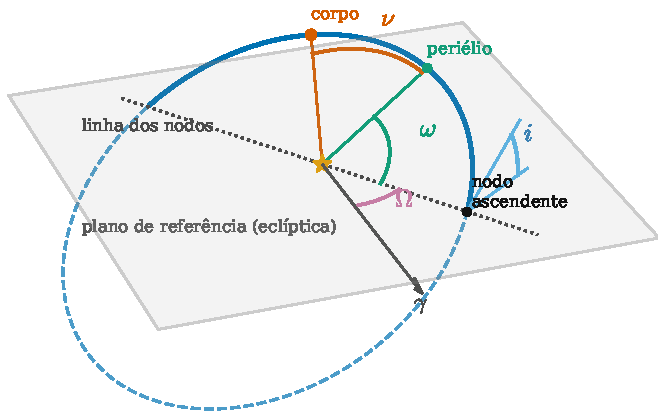
\includegraphics[width=0.85\textwidth]{elementos.pdf}
  \legend{$\Omega$: longitude do nodo ascendente, medida no plano de referência a partir da direção do equinócio $\gamma$; $i$: inclinação entre o plano da órbita e o de referência; $\omega$: argumento do periélio, medido no plano da órbita a partir do nodo; $\nu$: anomalia verdadeira. A parte tracejada da órbita está abaixo do plano de referência. O desenho é esquemático. Fonte: elaborada pelos autores.}
\end{figure}

Para levar um ponto da órbita ao espaço, escreve-se a posição na \emph{base perifocal}, com o eixo $x$ apontando para o periélio e o $y$ a $90^\circ$ no sentido do movimento, e aplica-se a rotação
\begin{equation}
  \vr = R_z(\Omega)\,R_x(i)\,R_z(\omega)\,
  \begin{pmatrix} x_P \\ y_P \\ 0 \end{pmatrix}.
  \label{eq:rotacao}
\end{equation}
A ordem importa. $R_z(\omega)$ gira o periélio a partir do nodo, $R_x(i)$ inclina o plano e $R_z(\Omega)$ leva o nodo à longitude certa. Trocar duas dessas rotações produz uma órbita plausível e errada, o tipo de erro que só aparece quando se compara com uma referência.

\paragraph{Elementos osculadores}

Num sistema real, a órbita de um planeta não é uma elipse fixa: os outros planetas a deformam devagar. Os \emph{elementos osculadores} num instante são os da elipse que o corpo seguiria se, a partir daquele instante, só o Sol existisse. Eles são calculados diretamente da posição e da velocidade relativas ao Sol:
\begin{align}
  a &= -\frac{\mu}{2\varepsilon} = \left(\frac{2}{r} - \frac{v^2}{\mu}\right)^{-1}, \label{eq:osc-a}\\
  \ve &= \frac{\vv\times\vh}{\mu} - \frac{\vr}{r}, \qquad e = |\ve|, \label{eq:osc-e}\\
  \cos i &= \frac{h_z}{|\vh|}, \label{eq:osc-i}
\end{align}
com $T$ dado pela \autoref{eq:terceiralei}. É o que o programa faz para desenhar o \emph{caminho previsto} de cada planeta e para alimentar o laboratório de Fourier.

\begin{licao}[: de onde se mede faz diferença]
A primeira versão do projeto (\autoref{sec:v-original}) calculava os elementos com a posição e a velocidade de cada planeta medidas a partir do \emph{baricentro} do Sistema Solar, que é o que a biblioteca Astropy devolve, mas usava nas fórmulas a gravidade do \emph{Sol}. As equações \eqref{eq:osc-a} a \eqref{eq:osc-i} valem para o estado \emph{relativo ao corpo central}. Como o Sol oscila em torno do baricentro cerca de 0,005 a 0,008\,UA, o erro era grande para os planetas internos: o semieixo de Mercúrio saía 1,7\,\% maior e a excentricidade de Vênus saía 0,0173 em vez de 0,0068, duas vezes e meia o valor correto. A correção é subtrair o estado do Sol antes de aplicar as fórmulas.
\end{licao}

\subsubsection{A equação de Kepler}\label{sec:kepler}

A segunda lei diz como a área varrida cresce com o tempo, mas não dá diretamente a posição em função do tempo. Para isso introduz-se a \emph{anomalia excêntrica} $E$, o ângulo medido do centro da elipse até a projeção do corpo sobre o círculo circunscrito de raio $a$ (\autoref{fig:anomalias}). Em termos de $E$, as coordenadas perifocais são
\begin{equation}
  x_P = a(\cos E - e),\qquad y_P = b\sin E = a\sqrt{1-e^2}\,\sin E,\qquad r = a(1 - e\cos E).
  \label{eq:perifocal}
\end{equation}

\begin{figure}[htb]
  \centering
  \caption{Anomalia excêntrica e anomalia verdadeira}
  \label{fig:anomalias}
  \begin{tikzpicture}[scale=1.5,>=Stealth]
    \def\semA{2.0}\def\exc{0.6}\def\angE{62}
    \pgfmathsetmacro{\semB}{\semA*sqrt(1-\exc*\exc)}
    \pgfmathsetmacro{\focC}{\semA*\exc}
    \pgfmathsetmacro{\angNu}{atan2(\semB*sin(\angE),\semA*cos(\angE)-\focC)}
    \coordinate (O) at (0,0);
    \coordinate (F) at (\focC,0);
    \coordinate (Q) at ({\semA*cos(\angE)},{\semA*sin(\angE)});
    \coordinate (P) at ({\semA*cos(\angE)},{\semB*sin(\angE)});
    \draw[gray!60,dashed] (O) circle (\semA);
    \draw[thick,blue!60!black] (O) ellipse ({\semA} and {\semB});
    \draw (-2.25,0) -- (2.35,0);
    \draw[gray] (O) -- (Q);
    \draw[gray,dotted] (Q) -- ({\semA*cos(\angE)},0);
    \draw[red!70!black,thick] (F) -- (P);
    \draw[->,gray!70!black] (0.45,0) arc (0:\angE:0.45);
    \node[font=\small] at ({0.62*cos(\angE/2)},{0.62*sin(\angE/2)}) {$E$};
    \draw[->,red!70!black] ($(F)+(0.32,0)$) arc (0:\angNu:0.32);
    \node[red!70!black,font=\small] at ($(F)+({0.5*cos(\angNu/2)},{0.5*sin(\angNu/2)})$) {$\nu$};
    \fill (O) circle (1pt) node[below,font=\scriptsize] {centro};
    \fill[orange!90!black] (F) circle (2pt) node[below=3pt,font=\scriptsize] {Sol (foco)};
    \fill[red!70!black] (P) circle (1.8pt) node[left,font=\scriptsize] {corpo};
    \fill[gray] (Q) circle (1.2pt) node[above right,font=\scriptsize] {projeção no círculo};
    \fill (\semA,0) circle (1pt) node[above right,font=\scriptsize] {periélio};
    \draw[<->] (0,-0.55) -- node[below,font=\scriptsize] {$ae$} (\focC,-0.55);
  \end{tikzpicture}
  \legend{O círculo tracejado tem raio $a$; a elipse é o círculo comprimido na vertical pelo fator $b/a$. Fonte: elaborada pelos autores.}
\end{figure}

A área do setor elíptico varrido desde o periélio, vista do foco, é a área do setor circular correspondente comprimida pelo fator $b/a$, menos o triângulo entre o centro e o foco:
\[
  A(E) = \frac{b}{a}\left(\frac{a^2E}{2} - \frac{a\cdot ae\,\sin E}{2}\right) = \frac{ab}{2}\,(E - e\sin E).
\]
Pela segunda lei, essa área cresce uniformemente no tempo e vale $\pi ab$ após um período. Logo $A = \pi ab\,(t-\tau)/T$, em que $\tau$ é o instante de passagem pelo periélio. Igualando as duas expressões e definindo a \emph{anomalia média} $M = n(t-\tau)$:
\begin{equation}
  \boxed{\;M = E - e\sin E\;}
  \label{eq:kepler}
\end{equation}
Esta é a equação de Kepler. Ela dá $M$ a partir de $E$ de forma explícita, mas o problema prático é o inverso: dado o tempo (e portanto $M$), achar $E$. Não há fórmula fechada com funções elementares, e a solução é numérica.

\paragraph{Solução pelo método de Newton}

Defina $f(E) = E - e\sin E - M$. O método de Newton itera
\begin{equation}
  E_{k+1} = E_k - \frac{f(E_k)}{f'(E_k)} = E_k - \frac{E_k - e\sin E_k - M}{1 - e\cos E_k}.
  \label{eq:newton-kepler}
\end{equation}
Para órbitas planetárias, com $e<0{,}21$, quatro ou cinco iterações a partir de $E_0 = M$ bastam para a precisão da máquina. O modo de criação de corpos do programa, porém, permite criar cometas com excentricidade próxima de 1, e nesse regime a escolha do ponto de partida importa. O programa usa o chute de \citeonline{danby1988},
\begin{equation}
  E_0 = M + 0{,}85\,e\,\sgn(\sin M),
\end{equation}
que coloca a primeira estimativa do lado certo do periélio. Como rede de segurança, se Newton não convergir o programa recorre à bisseção no intervalo $[M-e,\,M+e]$, que sempre contém a raiz porque $|E-M| = |e\sin E| \leq e$ e porque $f$ é monótona. A bisseção é lenta, mas nunca falha. O \autoref{cap:resultados} mede o número de iterações dos dois chutes (\autoref{fig:kepler-iteracoes}).

Com $E$ conhecido, a velocidade perifocal é
\begin{equation}
  \dot{x}_P = -\frac{\sqrt{\mu a}}{r}\sin E,\qquad \dot{y}_P = \frac{\sqrt{\mu a}}{r}\sqrt{1-e^2}\cos E,
\end{equation}
e a anomalia verdadeira, se necessária, sai da forma de meio ângulo
\[
  \tan\frac{\nu}{2} = \sqrt{\frac{1+e}{1-e}}\,\tan\frac{E}{2},
\]
calculada com a função \codigo{atan2} para não perder o quadrante.

\subsubsection{Referenciais e escala de tempo}

Todas as posições do simulador estão no referencial da eclíptica e equinócio de J2000, alinhado ao ICRF, com origem no baricentro do Sistema Solar \cite{park2021}. O tempo é o Tempo Dinâmico Baricêntrico (TDB), a variável independente das efemérides do JPL. A eclíptica de J2000 faz com o equador celeste o ângulo $\varepsilon_0 = 23{,}4392911^\circ$ (a obliquidade), usado para converter dados equatoriais, como os polos de rotação dos planetas publicados pela IAU \cite{archinal2018} e o catálogo de estrelas \cite{hoffleit1991}.

Os planetas são representados pelos \emph{baricentros dos seus sistemas}: o ponto chamado ``Terra'' é o centro de massa Terra--Lua, e o ponto ``Júpiter'' é o centro de massa de Júpiter com suas luas, cada um com a $GM$ do sistema inteiro. É assim que o próprio JPL integra os planetas, porque um sistema com luas se move, visto de longe, como um ponto de massa igual à soma das massas. O centro da Terra gira em torno do baricentro Terra--Lua a cerca de 4\,700\,km, o que na visão geral do sistema vale menos de um milésimo de pixel.

\subsubsection{O que o modelo físico não inclui}\label{sec:nao-inclui}

Ficam fora da integração:

\begin{itemize}
  \item a relatividade geral. O efeito mais conhecido é a precessão adicional do periélio de Mercúrio, de 43 segundos de arco por século \cite{will2018}. Em dez anos isso desloca o periélio de cerca de $2\times10^{-5}$\,rad, o que, multiplicado pela distância de Mercúrio ao Sol, dá da ordem de mil quilômetros. Esse valor é da ordem do patamar abaixo do qual o erro não cai ao reduzir o passo (\autoref{fig:trabalho-precisao}). Com o passo de 0,5 dia usado no programa, o erro de Mercúrio é maior que isso e vem sobretudo do truncamento do integrador;
  \item Plutão, os asteroides (inclusive Ceres e Vesta) e as luas como corpos dinâmicos separados;
  \item achatamento, marés e pressão de radiação.
\end{itemize}

Por isso os resultados se afastam devagar da efeméride do JPL, e o programa avisa o usuário. A versão 3D acrescenta treze luas, mas por outro método, sem integração (\autoref{sec:luas}).

% movido da seção 3 na Tarefa 6; a Tarefa 8 corta
\subsection{Integração numérica}\label{sec:integradores}

\begin{paracomecar}
O computador não resolve a equação do movimento de uma vez. Ele dá passos: sabendo onde cada planeta está e com que velocidade, calcula onde estará meio dia depois, e repete. O problema é que os pequenos erros de cada passo se somam e, com o tempo, deformam a órbita.
\end{paracomecar}

\subsubsection{O problema de um método ingênuo}

O método mais simples, o de Euler, atualiza posição e velocidade usando os valores do início do passo: $\vr_{k+1} = \vr_k + \Delta t\,\vv_k$, $\vv_{k+1} = \vv_k + \Delta t\,\va(\vr_k)$. Para uma órbita circular, cada passo leva o corpo pela tangente, ligeiramente para fora do círculo, e a energia cresce a cada volta. Depois de algumas centenas de órbitas, o planeta escapa. Métodos de ordem mais alta, como o Runge--Kutta clássico de quarta ordem (RK4), erram muito menos em cada passo, mas o erro de energia continua tendo sinal sistemático e cresce sem limite, só que mais devagar.

\subsubsection{Integradores simpléticos}

As equações de Newton para a gravitação têm estrutura hamiltoniana: o estado é um ponto no espaço de fase $(\vr,\vv)$ e a evolução exata preserva volumes nesse espaço (teorema de Liouville). Um integrador \emph{simplético} é um método cujo passo também preserva essa estrutura \cite{hairer2006}. A consequência prática, demonstrada pela análise de erro regressiva, é que a solução numérica de um integrador simplético é a solução \emph{exata} de um hamiltoniano ligeiramente modificado, $\tilde H = H + O(\Delta t^p)$. Como $\tilde H$ se conserva exatamente, a energia verdadeira $H$ apenas oscila em torno do valor inicial, com amplitude $O(\Delta t^p)$, sem crescimento secular, por tempos exponencialmente longos.

\subsubsection{Leapfrog (Verlet)}

O integrador simplético mais simples é o \emph{leapfrog}, ou Verlet de velocidade \cite{verlet1967}. Ele alterna meio impulso, um deslocamento inteiro e outro meio impulso:
\begin{align}
  \vv_{k+1/2} &= \vv_k + \tfrac12\Delta t\,\va(\vr_k), \nonumber\\
  \vr_{k+1}   &= \vr_k + \Delta t\,\vv_{k+1/2}, \label{eq:leapfrog}\\
  \vv_{k+1}   &= \vv_{k+1/2} + \tfrac12\Delta t\,\va(\vr_{k+1}). \nonumber
\end{align}
É de segunda ordem, simétrico no tempo (dar um passo com $-\Delta t$ desfaz exatamente o passo com $+\Delta t$, a menos do arredondamento) e custa uma avaliação de força por passo, porque $\va(\vr_{k+1})$ pode ser reaproveitada no passo seguinte. O simulador não faz esse reaproveitamento e gasta duas avaliações; nas comparações de custo da \autoref{sec:res-integradores} contamos uma, que é o custo do método. Denote por $S_2(\Delta t)$ esse passo.

\subsubsection{A composição de Yoshida}

\citeonline{yoshida1990} mostrou como construir métodos simpléticos de ordem mais alta compondo passos de um método simétrico de ordem 2. A versão de quarta ordem é
\begin{equation}
  S_4(\Delta t) = S_2(w_1\Delta t)\;S_2(w_0\Delta t)\;S_2(w_1\Delta t).
  \label{eq:yoshida}
\end{equation}
Os pesos saem de duas condições. A soma dos subpassos precisa dar o passo inteiro, $2w_1 + w_0 = 1$. E o termo de erro de terceira ordem, que em cada $S_2(h)$ é proporcional a $h^3$, precisa se cancelar: $2w_1^3 + w_0^3 = 0$. Resolvendo,
\begin{equation}
  w_1 = \frac{1}{2 - 2^{1/3}} \approx 1{,}35120719,\qquad
  w_0 = -\frac{2^{1/3}}{2 - 2^{1/3}} \approx -1{,}70241438.
  \label{eq:pesos-yoshida}
\end{equation}
O peso central é \emph{negativo}: o subpasso do meio anda para trás no tempo. O método resultante é simplético, simétrico, de quarta ordem e custa três avaliações de força por passo.

\begin{paraaprofundar}[: por que os pesos são escritos como números e não calculados]
O programa grava $w_1$ e $w_0$ como literais de 17 algarismos em vez de calcular $1/(2-\sqrt[3]{2})$ em tempo de execução. A razão é a reprodutibilidade: assim o valor não depende de a função de raiz cúbica de cada motor de JavaScript concordar com as demais no último bit. Um teste automatizado confere os literais contra a fórmula com tolerância de uma unidade na última casa.
\end{paraaprofundar}

\subsubsection{Passo fixo}

O simulador usa $S_4$ com passo \emph{fixo} de $\Delta t = 0{,}5$ dia, por duas razões independentes. Passo variável destrói a propriedade simplética, a menos de técnicas especiais. E com passo fixo a data exibida na tela é sempre exatamente $t_0 + k\cdot 0{,}5$ dia, sem arredondamento acumulado. O valor de meio dia foi escolhido por medição (\autoref{sec:res-integradores}).

\subsubsection{Interpolação para o desenho}

A física anda de meio em meio dia, mas a tela é redesenhada 60 ou 120 vezes por segundo. A 1 dia por segundo, isso daria dois saltos visíveis por segundo. O programa desenha uma posição intermediária entre dois estados integrados consecutivos usando a \emph{interpolação cúbica de Hermite}, que usa posição e velocidade nas duas pontas:
\begin{equation}
  \vr(\alpha) = h_{00}(\alpha)\,\vr_k + h_{10}(\alpha)\,\Delta t\,\vv_k + h_{01}(\alpha)\,\vr_{k+1} + h_{11}(\alpha)\,\Delta t\,\vv_{k+1},
  \qquad 0\le\alpha\le1,
  \label{eq:hermite}
\end{equation}
com $h_{00} = 2\alpha^3 - 3\alpha^2 + 1$, $h_{10} = \alpha^3 - 2\alpha^2 + \alpha$, $h_{01} = -2\alpha^3 + 3\alpha^2$ e $h_{11} = \alpha^3 - \alpha^2$. A curva resultante é contínua em posição e em velocidade nas fronteiras dos passos. Uma alternativa mais barata, extrapolar por Taylor a partir do estado atual, foi descartada por medição: em meio passo o termo de terceira ordem vale 213\,km em Mercúrio, 4\,\% do diâmetro do planeta, e isso aparecia como um tranco na fronteira de cada passo. A data escrita na tela é a do instante interpolado, $t_k + \alpha\Delta t$, de modo que o número na tela sempre corresponde ao desenho.

\subsection{Aritmética de ponto flutuante}\label{sec:float}

Computadores representam números reais com um número finito de algarismos binários, no padrão IEEE 754 \cite{ieee754,goldberg1991}. Em precisão dupla (\emph{float64}) há cerca de 16 algarismos decimais significativos; em precisão simples (\emph{float32}), cerca de 7. Toda a física do simulador roda em float64, e nessa precisão a posição de Netuno, a 30\,UA, fica quantizada em cerca de $10^{-15}\times 30\UA \approx 1\,\mathrm{mm}$.

As placas gráficas, porém, trabalham em float32, que em 30\,UA quantiza a centenas de quilômetros. O problema não é o valor em si, que seria invisível na tela, mas a \emph{subtração de dois números grandes e próximos}. A câmera a 30\,UA da origem olhando um planeta também a 30\,UA precisa calcular a diferença entre as duas posições, e em float32 essa diferença perde quase todos os algarismos significativos. A cena treme. A solução, descrita na \autoref{sec:origem-flutuante}, é fazer essa subtração em float64, na CPU, antes de enviar qualquer coisa para a placa.

\subsection{Escala de desenho}\label{sec:compressao}

Netuno está 77 vezes mais longe do Sol que Mercúrio. Numa tela que mostra o sistema inteiro em escala real, os quatro planetas internos ocupam uma área do tamanho de um dedo. O programa oferece, como opção desligada por padrão, o \emph{modo maquete}, que comprime as distâncias desenhadas por
\begin{equation}
  r_\text{desenho} = R\,\sqrt{r/R},\qquad R = 1\UA,
  \label{eq:compressao}
\end{equation}
preservando direções e mantendo a órbita da Terra inalterada (\autoref{fig:compressao}). A raiz foi preferida ao logaritmo porque é monótona, suave e vale zero em zero, enquanto o logaritmo leva o centro a $-\infty$ e exige um piso arbitrário. A razão entre o planeta mais distante e o mais próximo cai de 77:1 para 8,8:1.

\begin{figure}[htb]
  \centering
  \caption{A compressão de distâncias do modo maquete}
  \label{fig:compressao}
  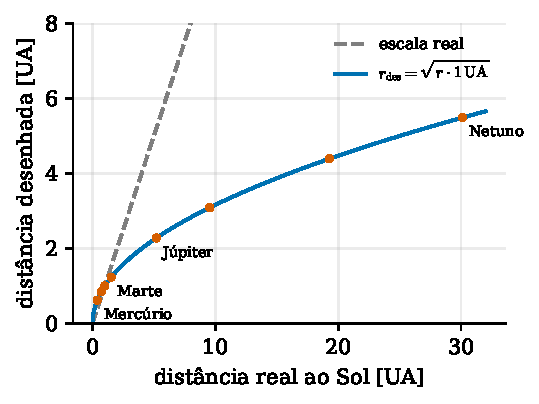
\includegraphics[width=0.62\textwidth]{compressao.pdf}
  \legend{Os pontos marcam os semieixos dos oito planetas. Fonte: elaborada pelos autores.}
\end{figure}

A compressão altera só a coordenada de desenho, nunca o estado físico. A iluminação continua usando a distância real, para que Netuno, desenhado a 5,5\,UA do Sol, não receba trinta vezes mais luz do que recebe. Com a compressão ligada, a tela avisa por escrito.

\subsection{Implementação: três gerações de um mesmo programa}\label{cap:implementacao}

O projeto passou por três versões, cada uma nascida das limitações da anterior (\autoref{fig:linha-do-tempo}). Este capítulo descreve o que cada uma fez, como a física e a matemática dos capítulos anteriores viraram código e por que algumas decisões foram tomadas. Os algoritmos aparecem em pseudocódigo; o código real está no repositório indicado no \autoref{ap:reproducao}.

\begin{figure}[htb]
  \centering
  \caption{As três gerações do projeto}
  \label{fig:linha-do-tempo}
  \begin{tikzpicture}[
      node distance=0.55cm and 0.5cm,
      caixa/.style={draw,rounded corners=2pt,align=left,font=\scriptsize,text width=4.1cm,inner sep=4pt},
      titulo/.style={font=\small\bfseries,align=center},
      >=Stealth]
    \node[caixa,fill=gray!8] (tcc) {\textbf{TCC de referência} (2016)\\ Maple + Gnuplot\\ epiciclos de Copérnico $\times$ série de Fourier, 5 planetas};
    \node[caixa,fill=blue!6,right=of tcc] (v1) {\textbf{1. Versão original}\\ Python, NumPy, Matplotlib, Astropy\\ elipse de Kepler e reconstrução por Fourier, um gráfico por planeta};
    \node[caixa,fill=green!6,below=of v1] (v2) {\textbf{2. Versão 2D}\\ Python, NumPy, Pygame\\ 9 corpos integrados (Yoshida 4), efeméride do JPL, laboratório de Fourier, testes automatizados};
    \node[caixa,fill=orange!8,left=of v2] (v3) {\textbf{3. Versão 3D}\\ TypeScript, three.js (WebGPU/WebGL2), Preact\\ mesma física, 13 luas, texturas, epiciclos complexos, sandbox, 43 funcionalidades com prova};
    \draw[->,thick,gray] (tcc) -- node[above,font=\tiny]{ideia} (v1);
    \draw[->,thick,gray] (v1) -- node[right,font=\tiny,align=left]{física em vez de\\fórmula fixa} (v2);
    \draw[->,thick,gray] (v2) -- node[above,font=\tiny,align=center]{desenho novo,\\física portada} (v3);
  \end{tikzpicture}
  \legend{Fonte: elaborada pelos autores.}
\end{figure}

\subsubsection{Versão original: a elipse e a série}\label{sec:v-original}

A primeira versão, em Python, tem cerca de 300 linhas e faz uma coisa só: dado um planeta e um número de termos, desenha a elipse de Kepler e a aproximação por série de Fourier no mesmo gráfico do Matplotlib. Ela reproduz, com ferramentas modernas, o experimento numérico de \citeonline{farias2016}.

O passo que essa versão acrescentou ao TCC foi obter os elementos orbitais de uma efeméride em vez de copiá-los de uma tabela. A biblioteca Astropy \cite{astropy2022} fornece posição e velocidade de cada planeta na época J2000, e as equações \eqref{eq:osc-a} a \eqref{eq:osc-i} dão $a$, $e$ e $T$. Foi aqui que apareceu o erro de referencial descrito na lição do \autoref{sec:elementos}: os vetores vinham do baricentro, e a excentricidade de Vênus saía duas vezes e meia maior que a real. A \autoref{tab:v1-baricentro} mostra o efeito, medido no próprio código depois da correção.

\begin{table}[htb]
  \centering
  \caption{Elementos calculados na versão original, antes e depois da correção de referencial}
  \label{tab:v1-baricentro}
  \begin{tabular}{lccc}
    \toprule
    Planeta & $a$ com vetores baricêntricos (UA) & $a$ corrigido (UA) & referência (UA) \\
    \midrule
    Mercúrio & 0,39378 \;(+1,73\,\%) & 0,38710 & 0,38710 \\
    Vênus    & 0,73868 \;(+2,12\,\%) & 0,72332 & 0,72333 \\
    Terra    & 0,99657 \;($-$0,34\,\%) & 1,00000 & 1,00000 \\
    Marte    & 1,50514 \;($-$1,22\,\%) & 1,52376 & 1,52371 \\
    \bottomrule
  \end{tabular}
  \legend{Época J2000, efeméride embutida do Astropy. A excentricidade de Vênus passou de 0,01734 para 0,00677. Fonte: documentação do módulo \arquivo{utils/lib.py} da versão original.}
\end{table}

Essa versão também amostrava a elipse \emph{em ângulo}, e não no tempo, o que, como vimos no \autoref{sec:param-tempo}, dá coeficientes de outra função. Ela permanece no repositório como referência científica e como registro do ponto de partida.

\subsubsection{Versão 2D: a física no lugar da fórmula}\label{sec:v2d}

A segunda versão deixou de desenhar uma elipse a partir de uma fórmula e passou a \emph{simular} o Sistema Solar: o Sol e os oito planetas se atraem mutuamente pela \autoref{eq:nbody}, todos no mesmo relógio, a partir das posições e velocidades medidas pelo JPL para 1º de janeiro de 2026. A elipse passou a ser uma consequência da simulação: ao abrir o laboratório de Fourier, o programa calcula os elementos osculadores do planeta naquele instante e a decompõe.

\begin{figure}[htb]
  \centering
  \caption{A versão 2D, em Python e Pygame}
  \label{fig:v2}
  \begin{subfigure}[b]{0.49\textwidth}
    \centering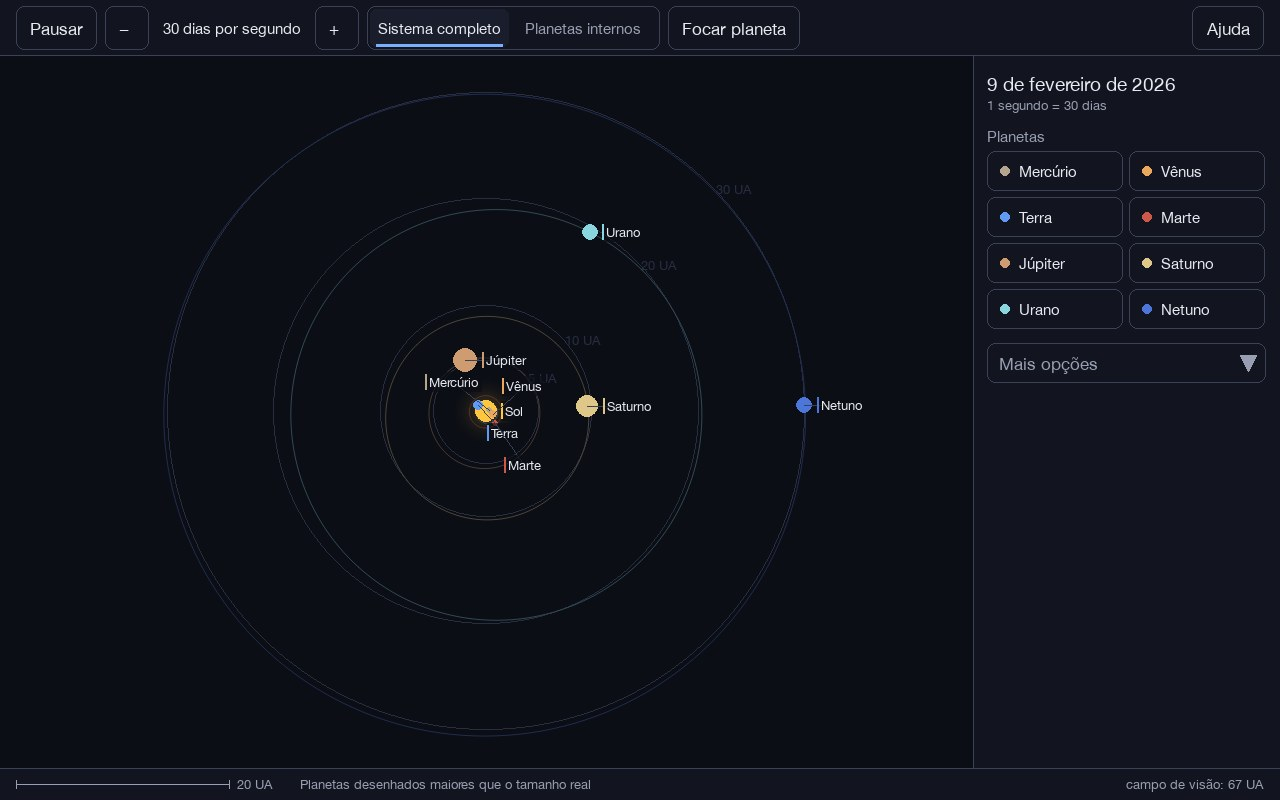
\includegraphics[width=\textwidth]{v2_visao_geral.jpg}
    \caption{Visão geral, em escala real}
  \end{subfigure}\hfill
  \begin{subfigure}[b]{0.49\textwidth}
    \centering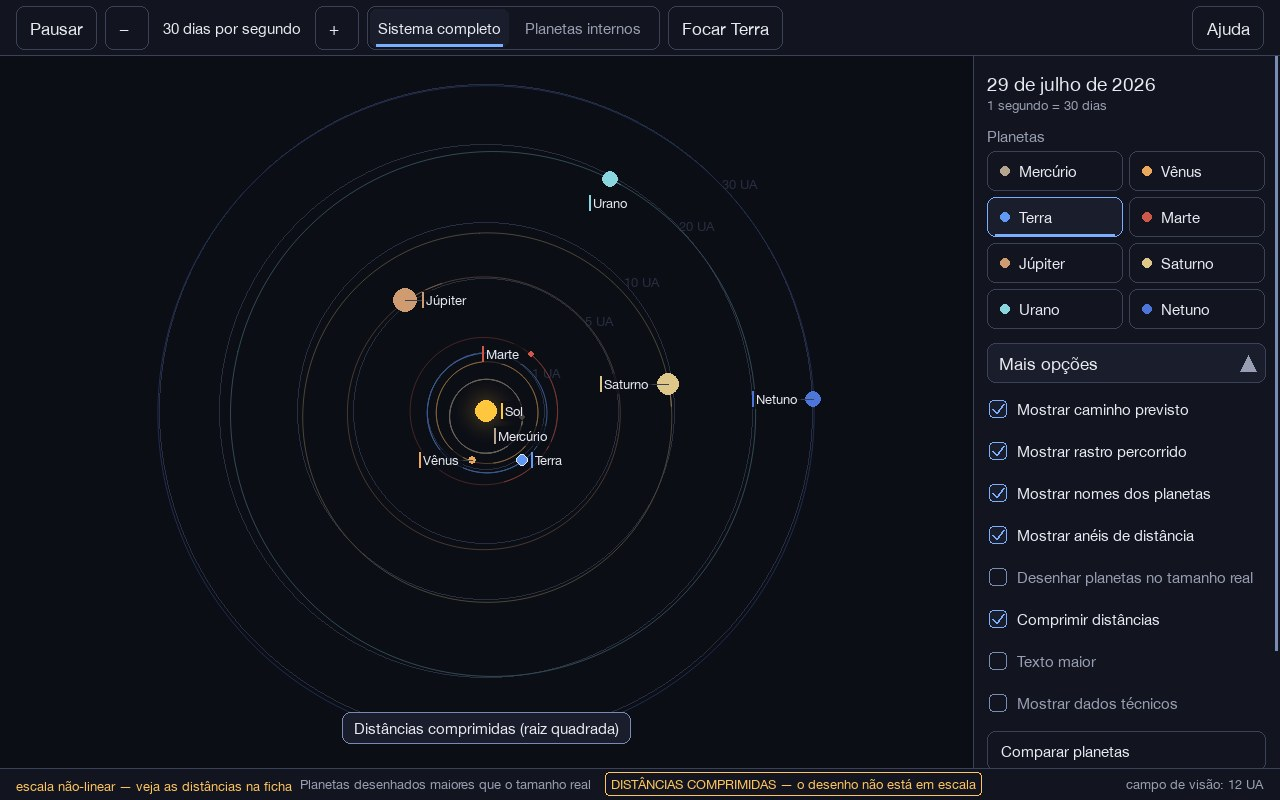
\includegraphics[width=\textwidth]{v2_comprimida.jpg}
    \caption{Com distâncias comprimidas}
  \end{subfigure}\\[4pt]
  \begin{subfigure}[b]{0.49\textwidth}
    \centering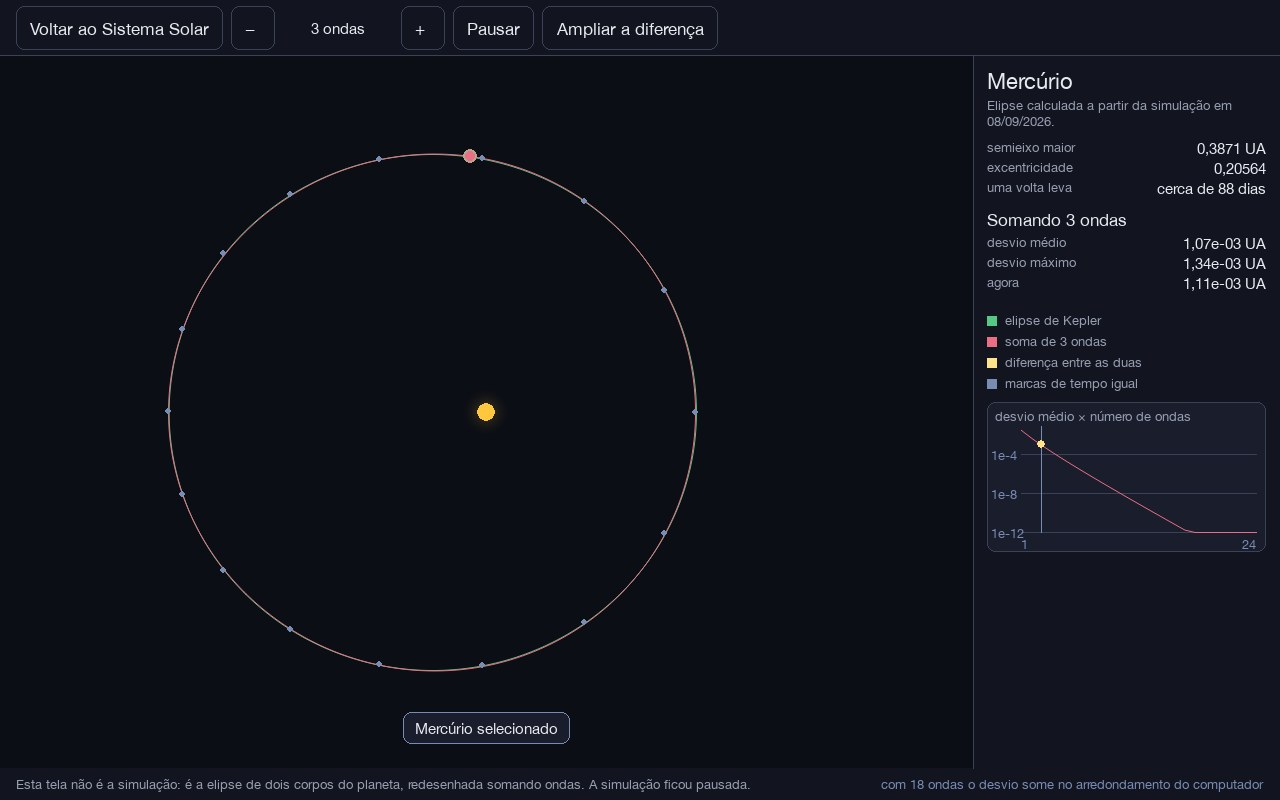
\includegraphics[width=\textwidth]{v2_laboratorio.jpg}
    \caption{Laboratório: Mercúrio com 3 ondas}
  \end{subfigure}\hfill
  \begin{subfigure}[b]{0.49\textwidth}
    \centering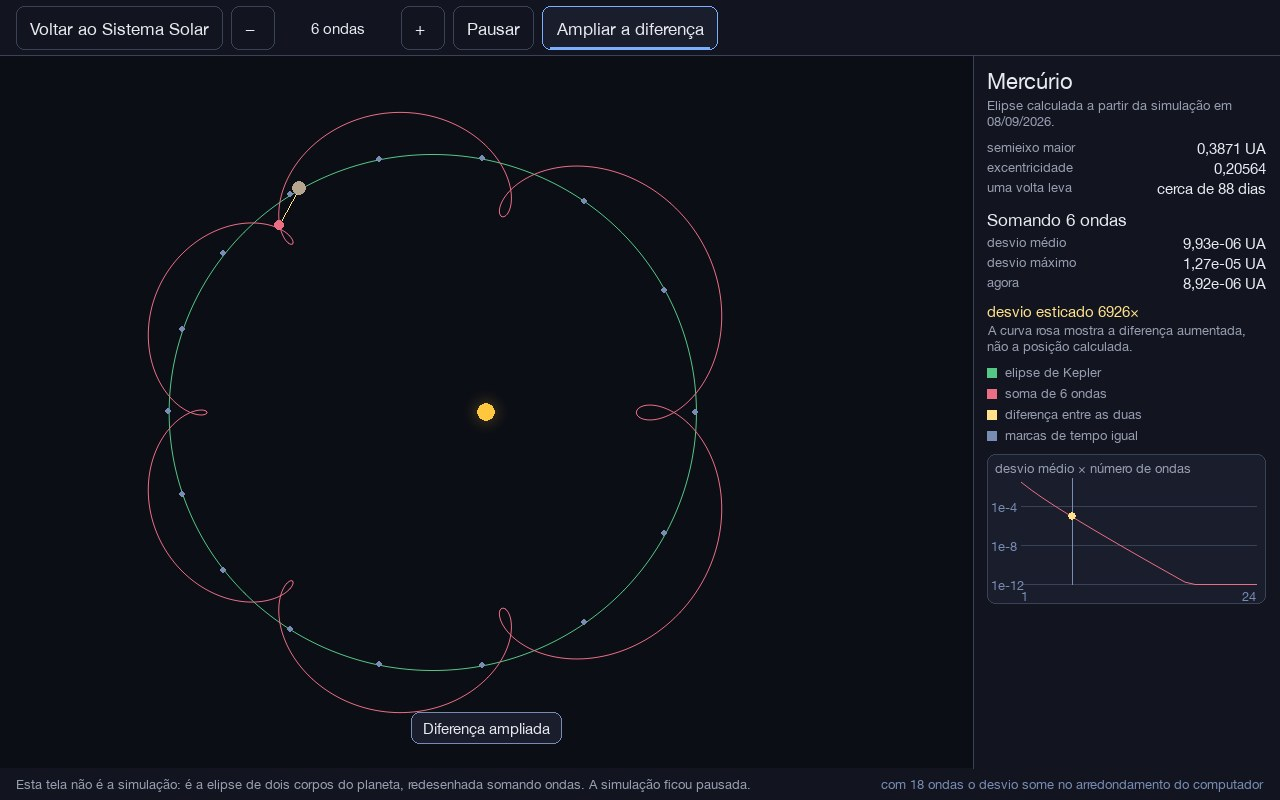
\includegraphics[width=\textwidth]{v2_laboratorio_ampliado.jpg}
    \caption{Diferença ampliada 6\,926 vezes}
  \end{subfigure}
  \legend{Em (b) a tela avisa por escrito que o desenho não está em escala. Em (d) a curva rosa mostra a diferença entre a série com 6 ondas e a elipse, multiplicada para ficar visível; o gráfico à direita mostra a convergência. Fonte: capturas do programa.}
\end{figure}

\paragraph{Dados de partida}

Um roteiro separado, \arquivo{ferramentas/gerar\_efemeride.py}, consulta uma única vez a API do JPL Horizons \cite{giorgini1996} e grava num arquivo JSON:

\begin{itemize}
  \item posição e velocidade de cada corpo em 1/1/2026, 0h TDB, relativas ao baricentro do Sistema Solar, no referencial da eclíptica J2000 (o Horizons informa a efeméride DE441 como origem);
  \item os parâmetros gravitacionais $GM$ do cabeçalho da efeméride DE440 \cite{park2021};
  \item os raios médios dos corpos;
  \item posições de validação em $-100$, $-10$, $+1$, $+10$ e $+100$ anos, que os testes usam para medir o erro;
  \item a procedência de cada número.
\end{itemize}

O programa em si \emph{nunca acessa a internet}: o arquivo é copiado junto. A versão 3D usa o mesmo arquivo, byte a byte, o que mantém válida a mesma tabela de erro.

\paragraph{Integração e relógio}

O integrador é o Yoshida de quarta ordem com passo fixo de 0,5 dia (\autoref{sec:integradores}), com o leapfrog mantido como referência independente nos testes. A força é calculada pelo \autoref{alg:forca} e o passo pelo \autoref{alg:yoshida}.

\begin{algorithm}[htb]
  \caption{Aceleração gravitacional mútua de $N$ corpos}\label{alg:forca}
  \KwIn{posições $\vr_1,\dots,\vr_N$ e parâmetros $\mu_1,\dots,\mu_N$}
  \KwOut{acelerações $\va_1,\dots,\va_N$}
  $\va_i \leftarrow \vetor{0}$ para todo $i$\;
  \For{$i\leftarrow 1$ \KwTo $N-1$}{
    \For{$j\leftarrow i+1$ \KwTo $N$}{
      $\vetor{d} \leftarrow \vr_j - \vr_i$;\quad $s \leftarrow 1/(|\vetor{d}|^2\,|\vetor{d}|)$\Com*[r]{uma raiz por par}
      $\va_i \leftarrow \va_i + \mu_j\, s\,\vetor{d}$\Com*[r]{$j$ puxa $i$}
      $\va_j \leftarrow \va_j - \mu_i\, s\,\vetor{d}$\Com*[r]{terceira lei}
    }
  }
\end{algorithm}

\begin{algorithm}[htb]
  \caption{Um passo de Yoshida de quarta ordem}\label{alg:yoshida}
  \KwIn{estado $(\vr,\vv)$, passo $\Delta t$}
  $w_1 \leftarrow 1{,}3512071919596578$;\quad $w_0 \leftarrow -1{,}7024143839193155$\;
  \ForEach{$w \in (w_1, w_0, w_1)$}{
    $\vr \leftarrow \vr + \tfrac12 w\,\Delta t\,\vv$\Com*[r]{meio deslocamento}
    $\va \leftarrow$ \textsc{Aceleração}$(\vr)$\Com*[r]{\autoref{alg:forca}}
    $\vv \leftarrow \vv + w\,\Delta t\,\va$\Com*[r]{impulso}
    $\vr \leftarrow \vr + \tfrac12 w\,\Delta t\,\vv$\Com*[r]{meio deslocamento}
  }
\end{algorithm}

Quando a pessoa pede, por exemplo, 3\,650 dias simulados por segundo, cada quadro de tela precisa de dezenas de passos. Se a máquina não der conta, há três saídas ruins: aumentar o passo (a física piora sem aviso), acumular a dívida (o programa trava tentando alcançar) ou pular passos (a data na tela deixa de corresponder ao desenho). O simulador mede a velocidade da máquina na abertura, oferece só as velocidades que ela sustenta, entrega em cada quadro os passos que cabem no orçamento, \emph{descarta} o excedente e avisa na tela que está atrasado (\autoref{alg:relogio}). A data mostrada é sempre $t_0 + k\cdot0{,}5$ dia exatos.

\begin{algorithm}[htb]
  \caption{Avanço do relógio dentro do orçamento do quadro (simplificado)}\label{alg:relogio}
  \KwIn{tempo real decorrido $\delta$, velocidade pedida $s$ (dias/segundo), orçamento $B$ (ms), cronômetro injetado}
  $\text{dívida} \leftarrow \text{dívida} + s\,\delta$\;
  $k \leftarrow 0$;\quad $t_\text{ini} \leftarrow$ cronômetro()\;
  \While{$\text{dívida} \geq \Delta t$ \textbf{e} cronômetro()$ - t_\text{ini} < B$}{
    \textsc{PassoYoshida}$(\Delta t)$;\quad $\text{dívida} \leftarrow \text{dívida} - \Delta t$;\quad $k \leftarrow k+1$\;
  }
  \If{$\text{dívida} \geq \Delta t$}{
    $\text{atrasado} \leftarrow$ verdadeiro;\quad $\text{dívida} \leftarrow \text{dívida} \bmod \Delta t$\Com*[r]{descarta, não acumula}
  }
  \Return $k$ passos dados, atrasado\;
\end{algorithm}

\paragraph{Laboratório de Fourier}

O laboratório pausa a simulação, calcula os elementos osculadores do corpo escolhido, gera a elipse de Kepler com 720 pontos igualmente espaçados no tempo (resolvendo a equação de Kepler para cada um) e calcula os coeficientes até 24 harmônicos. Mostrar mais ou menos harmônicos é só truncar a soma, sem recalcular, e por isso o controle responde na hora. A tela mostra o desvio médio e máximo e um gráfico de convergência (\autoref{fig:v2}c e d).

\paragraph{Limites declarados na Ajuda}

A partir da versão 2D, a Ajuda do programa traz três blocos: \emph{o que calcula}, \emph{o que a tela simplifica} e \emph{o que o modelo não inclui}. Os planetas são desenhados maiores que o real, e uma opção mostra o tamanho verdadeiro, em que eles somem. A escala comprimida é avisada por escrito, e a régua de distância é trocada pelo aviso, porque uma régua linear sobre uma escala não linear daria leituras erradas. O erro contra o JPL aparece em números.

\begin{licao}[: a câmera que nunca alcançava o planeta]
A câmera que acompanha um planeta usava amortecimento exponencial em direção à posição do corpo. Esse método nunca alcança um alvo em movimento: estabiliza a uma distância proporcional à velocidade do alvo. Medimos 11 pixels de atraso com Marte a 30 dias por segundo e 237 pixels a 3\,650. A solução foi dar prazo à transição, 0,45\,s de animação, e depois prender a câmera ao corpo. Um defeito assim só aparece quando alguém mede, porque a olho a câmera ``parece'' seguir o planeta.
\end{licao}

\subsubsection{Versão 3D: a mesma física, outro desenho}\label{sec:v3d}

A terceira versão reescreveu o programa em TypeScript para rodar no navegador, com three.js \cite{threejs} desenhando em WebGPU \cite{webgpu} e, como alternativa, em WebGL2. A física, os dados e os textos vieram da versão 2D, e o contrato do projeto foi explícito: a versão 3D tinha de entregar as 43 funcionalidades da 2D antes de qualquer novidade (\autoref{sec:contrato}). O código tem cerca de 15\,000 linhas em 86 arquivos, e os testes outras 10\,000.

\begin{figure}[htb]
  \centering
  \caption{A versão 3D}
  \label{fig:v3-galeria}
  \begin{subfigure}[b]{0.49\textwidth}
    \centering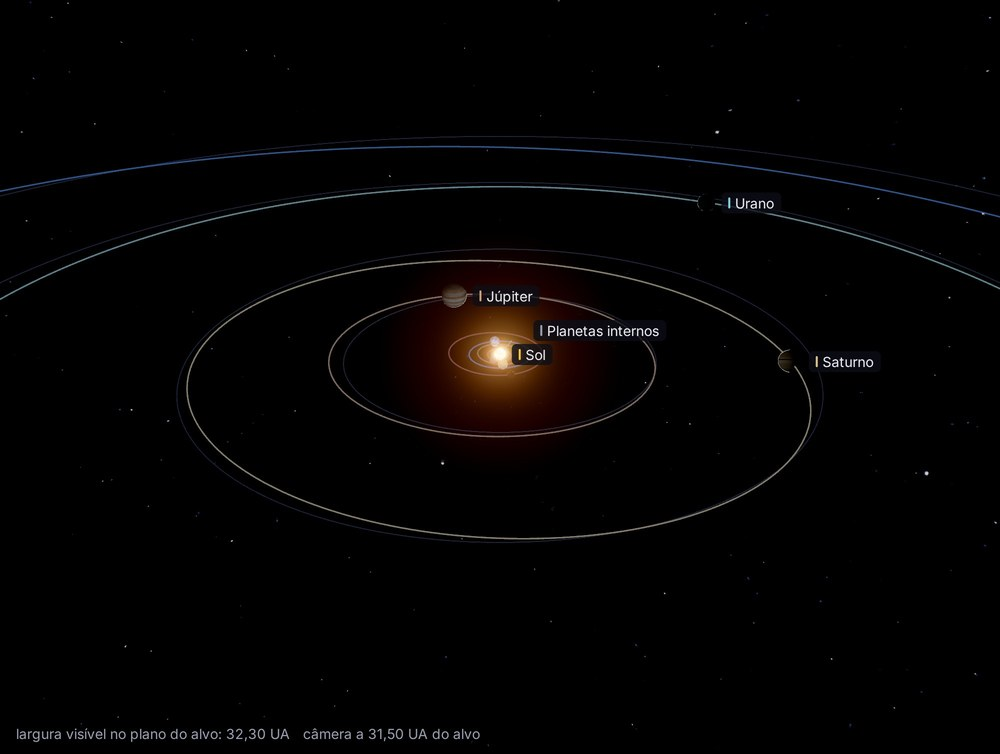
\includegraphics[width=\textwidth]{v3_visao_geral.jpg}
    \caption{Visão geral, a 31,5\,UA}
  \end{subfigure}\hfill
  \begin{subfigure}[b]{0.49\textwidth}
    \centering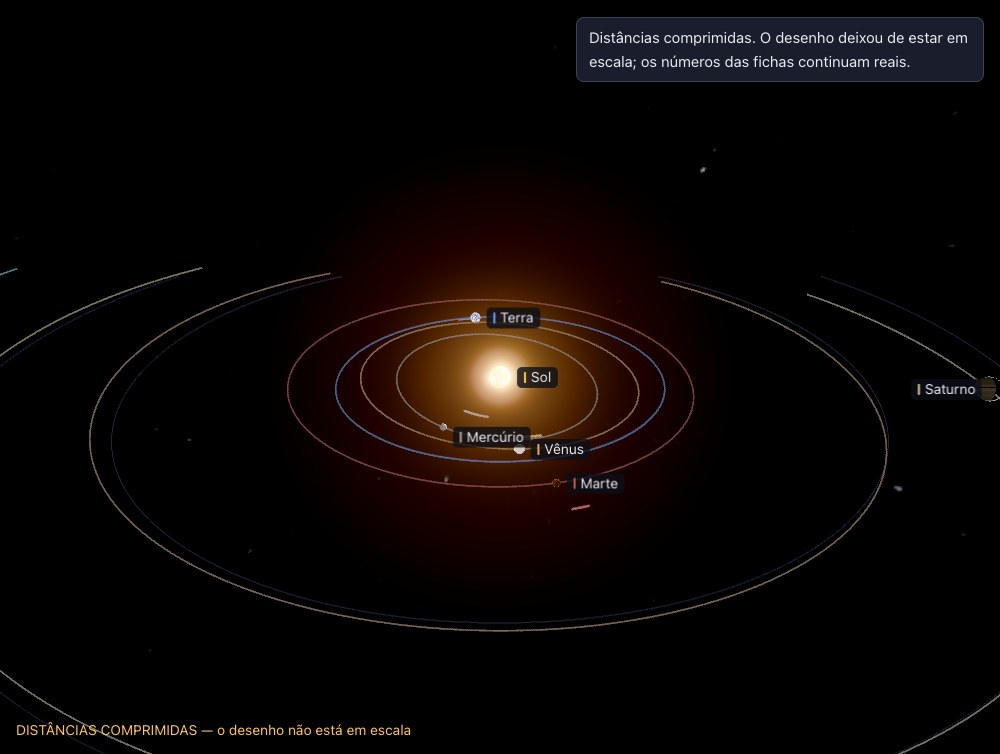
\includegraphics[width=\textwidth]{v3_maquete.jpg}
    \caption{Modo maquete, com o aviso}
  \end{subfigure}\\[4pt]
  \begin{subfigure}[b]{0.49\textwidth}
    \centering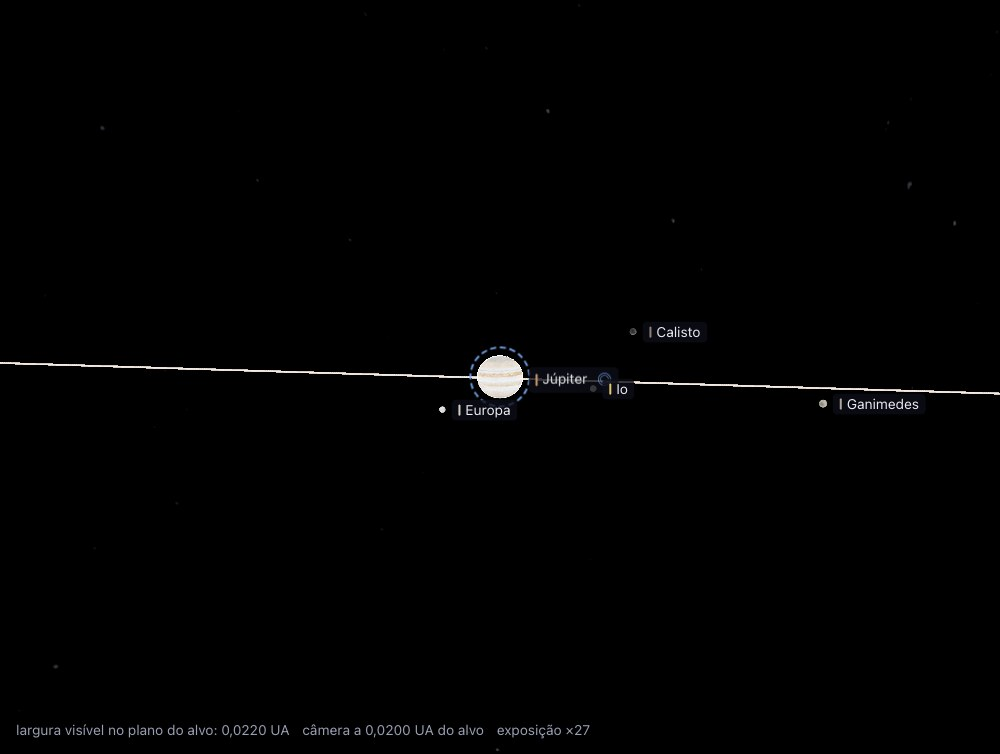
\includegraphics[width=\textwidth]{v3_jupiter_e_as_galileanas.jpg}
    \caption{Júpiter e as luas galileanas}
  \end{subfigure}\hfill
  \begin{subfigure}[b]{0.49\textwidth}
    \centering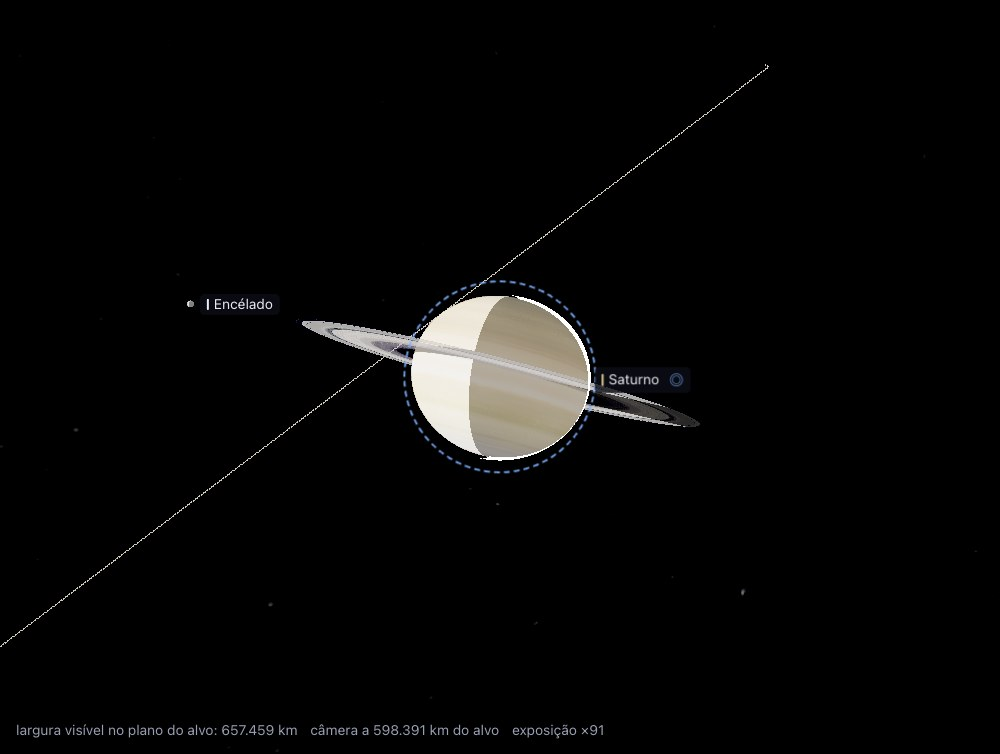
\includegraphics[width=\textwidth]{v3_saturno_e_os_aneis.jpg}
    \caption{Saturno, anéis e as duas sombras}
  \end{subfigure}\\[4pt]
  \begin{subfigure}[b]{0.49\textwidth}
    \centering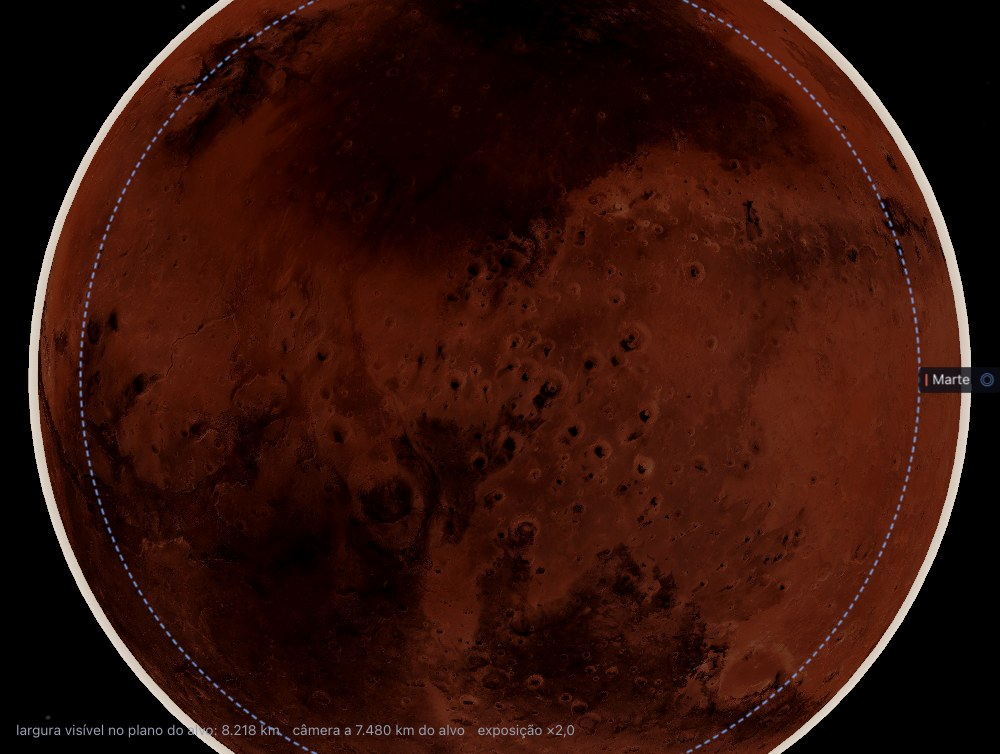
\includegraphics[width=\textwidth]{v3_marte_em_orbita_baixa.jpg}
    \caption{Marte a três raios, textura 8K}
  \end{subfigure}\hfill
  \begin{subfigure}[b]{0.49\textwidth}
    \centering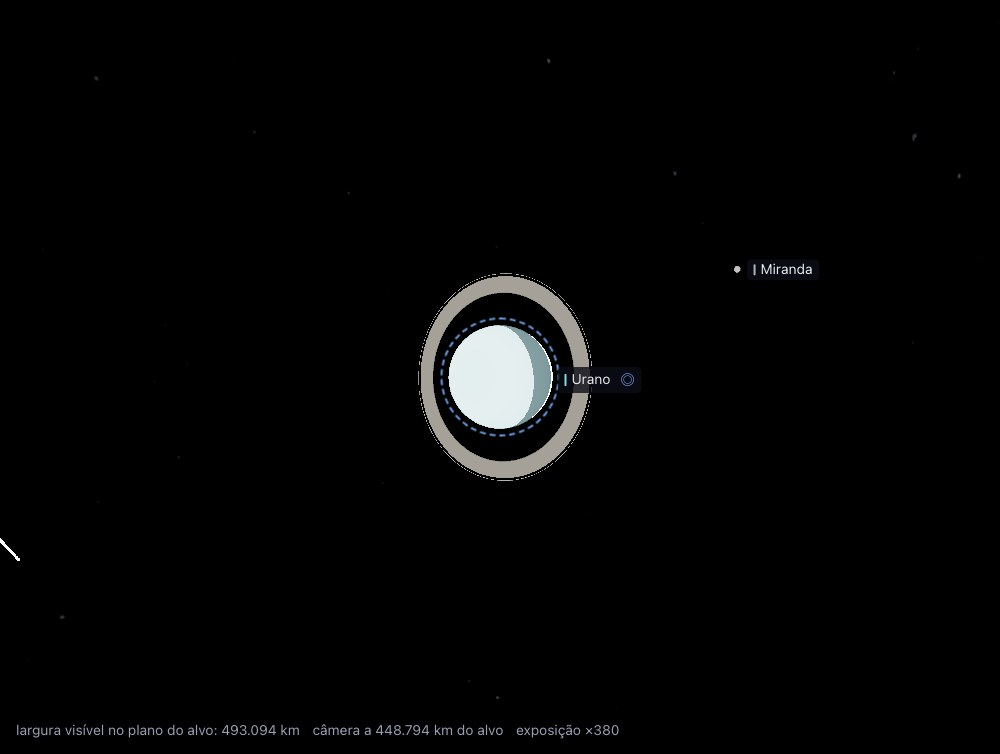
\includegraphics[width=\textwidth]{v3_urano_deitado.jpg}
    \caption{Urano, com eixo inclinado a $98^\circ$}
  \end{subfigure}
  \legend{Cenas de referência usadas pelos testes visuais automatizados. A barra inferior de cada cena traz a largura visível, a distância da câmera e o fator de exposição, escritos pelo próprio programa. Fonte: capturas do programa.}
\end{figure}

\paragraph{Arquitetura em camadas}

O código é dividido em camadas com regras de dependência verificadas automaticamente (\autoref{fig:camadas}). A regra central é que o núcleo físico não enxerga nada além de si mesmo: não sabe que existe uma tela, não lê o relógio do sistema, não sorteia números e não acessa a rede. Isso garante que a física possa ser testada sem navegador e que seja determinística. Sete regras, escritas num arquivo de configuração da ferramenta \emph{dependency-cruiser}, travam a compilação se alguém importar uma camada proibida. Uma regra de \emph{lint} proíbe ainda, dentro do núcleo, as quatro funções globais que quebrariam essas garantias em silêncio: \codigo{Math.random}, \codigo{Date.now}, \codigo{performance} e \codigo{fetch}.

\begin{figure}[htb]
  \centering
  \caption{Camadas da versão 3D e o sentido das dependências}
  \label{fig:camadas}
  \begin{tikzpicture}[
      node distance=0.35cm and 0.6cm,
      cam/.style={draw,rounded corners=2pt,font=\scriptsize,align=center,minimum width=2.6cm,minimum height=0.85cm,inner sep=3pt},
      >=Stealth]
    \node[cam,fill=blue!8] (nucleo) {\textbf{nucleo/}\\física pura};
    \node[cam,fill=gray!10,below=of nucleo] (contratos) {\textbf{contratos/}\\tipos compartilhados};
    \node[cam,fill=green!8,right=1.2cm of nucleo] (dados) {\textbf{dados/}\\fatos com procedência};
    \node[cam,fill=yellow!12,above=of nucleo] (app) {\textbf{app/}\\ações, laço do quadro};
    \node[cam,fill=orange!10,left=1.2cm of app] (cena) {\textbf{cena/}\\three.js};
    \node[cam,fill=red!6,right=1.2cm of app] (interface) {\textbf{interface/}\\Preact};
    \node[cam,fill=purple!6,above=of app] (rotulos) {\textbf{rotulos/}\\geometria de tela};
    \draw[->] (app) -- (nucleo);
    \draw[->] (app) -- (dados);
    \draw[->] (app) -- (cena);
    \draw[->] (app) -- (interface);
    \draw[->] (app) -- (rotulos);
    \draw[->] (dados) -- (contratos);
    \draw[->] (nucleo) -- (contratos);
    \draw[->] (cena) |- (contratos);
    \draw[->] (interface) |- (contratos);
  \end{tikzpicture}
  \legend{Uma seta de A para B significa ``A pode importar B''. O núcleo e os dados não importam nenhuma camada de desenho; a cena não importa a aplicação, e por isso não consegue abrir uma janela nem disparar uma ação. Fonte: elaborada pelos autores a partir de \arquivo{ARQUITETURA.md}.}
\end{figure}

\paragraph{A origem flutuante}\label{sec:origem-flutuante}

Como discutido na \autoref{sec:float}, a placa gráfica trabalha em float32, e a subtração entre a posição da câmera e a de um corpo, ambas grandes, destrói a precisão. A solução adotada é a \emph{origem flutuante}: a câmera fica sempre na origem da cena, e a posição de cada corpo \emph{relativa à câmera} é calculada em float64, na CPU, antes de ir para a placa. A coluna de translação da matriz de vista é zero por construção. A alternativa ingênua, enviar as posições absolutas em float32, quantizaria a posição em cerca de 270\,km a 30\,UA e 13\,km a 1,5\,UA, e Fobos, com cerca de 11\,km de raio, ficaria do tamanho do quantum de posição do próprio planeta.

\paragraph{Fatias de profundidade}

Entre a superfície de um planeta vista de perto (cerca de 1\,km) e a órbita de Netuno ($4{,}5\times10^9$\,km) há nove ordens de grandeza. Um \emph{z-buffer} de 24 bits, que guarda a profundidade de cada pixel para decidir o que fica na frente, não distingue nada nessa faixa. O programa desenha a cena em \emph{fatias de profundidade}: a mais distante primeiro, depois limpa o z-buffer e desenha a mais próxima por cima, cada fatia com razão entre o plano distante e o próximo de no máximo $10^5$. A técnica não depende de recursos específicos do renderizador e funciona igualmente nos dois backends.

\paragraph{Luz, superfície e céu}

A iluminação tem uma única fonte, pontual, no Sol. A borda entre dia e noite, o \emph{terminador}, recebe uma penumbra da largura angular do disco solar visto do planeta,
\begin{equation}
  s = \frac{R_\odot}{d},\qquad
  \text{luz} = \operatorname{smoothstep}\bigl(-s,\,s,\,\hat{\vetor{n}}\cdot\hat{\vetor{l}}\bigr),
\end{equation}
em que $d$ é a distância real ao Sol, $\hat{\vetor{n}}$ a normal da superfície e $\hat{\vetor{l}}$ a direção do Sol. Sem ela o terminador vira uma linha dura que denuncia a computação gráfica. O lado noturno recebe um piso de 14\,\% da luz do meio-dia, um ajuste visual avisado na Ajuda: sem ele, Marte visto com o Sol atrás era um disco preto, e o programa existe para mostrar como os planetas são.

A orientação de cada corpo segue as constantes de rotação da IAU \cite{archinal2018}: polo norte em ascensão reta e declinação $(\alpha_0,\delta_0)$ e meridiano principal $W = W_0 + \dot W d$. Como a simulação roda na eclíptica, a matriz completa é $R_x(-\varepsilon_0)\,R_z(\alpha_0 + 90^\circ)\,R_x(90^\circ - \delta_0)\,R_z(W)$. As texturas de superfície vêm do Solar System Scope e, para cinco luas, dos mosaicos de imageamento real Voyager, Galileo e Cassini do USGS. O céu de fundo é o \emph{Yale Bright Star Catalogue} \cite{hoffleit1991}: 8\,404 estrelas na posição correta, com brilho dado pela magnitude, $L\propto 10^{-0{,}4(V-6{,}5)}$, e cor de corpo negro dada pela temperatura de cada uma.

\begin{licao}[: a esfera girada noventa graus]
O gerador de esferas do three.js constrói os polos sobre o eixo $y$, enquanto todo o resto do programa trata $z$ como polo. Durante várias fases, a textura de cada planeta esteve desenhada com o polo sobre o equador do corpo. Nenhum teste acusava: o teste de orientação media a \emph{matriz}, que sempre esteve certa, e as imagens de referência tinham sido gravadas já com o defeito, de modo que travavam o erro em vez de denunciá-lo. O defeito foi achado por uma pergunta que nenhum teste fazia, onde a textura cai na geometria, e passou a ter um teste com resposta conhecida: como a Lua tem rotação sincronizada, da Terra vê-se sempre a face com os grandes mares escuros. A área escura medida na imagem só sai certa se matriz, geometria, meridiano e mapa estiverem certos ao mesmo tempo.
\end{licao}

\paragraph{As luas}\label{sec:luas}

A versão 3D acrescenta treze luas: a Lua, Fobos, Deimos, as quatro galileanas, Encélado, Titã, Titânia, Oberon, Miranda e Tritão. Elas \emph{não} entram no integrador. Io dá uma volta em 1,77 dia; com passo de meio dia seriam três passos e meio por órbita, regime em que nenhum integrador de passo fixo funciona. Reduzir o passo global para atender a Io custaria o desempenho de todo o resto e alteraria a camada dinâmica validada contra o JPL.

As luas são propagadas analiticamente pela \autoref{sec:kepler}, a partir dos elementos médios publicados pelo JPL, com taxas seculares de precessão do nodo e do periastro:
\begin{equation}
  M(t) = M_0 + \dot M\,t,\qquad
  \Omega(t) = \Omega_0 + \dot\Omega\,t,\qquad
  \omega(t) = \omega_0 + \dot\omega\,t.
\end{equation}
Elas não puxam nada e não alteram o estado dos nove corpos. O preço é um erro limitado, medido numa janela de vinte anos que os dados de ajuste nunca viram (\autoref{sec:res-luas}). Ao gerar esses dados, apareceram três problemas que a página do JPL não menciona:

\begin{itemize}
  \item a coluna de período não é o período sideral de todas as luas. Em Io ela difere 0,36\,\% do período medido, o que em um ano desloca a lua 270 graus. O programa mede o período casando a fase entre duas janelas de vetores do Horizons separadas por dezesseis anos;
  \item cada lua usa um plano de referência: a eclíptica (só a Lua), o plano de Laplace (a maioria) ou o equador do planeta (as luas de Urano). Misturar os planos põe a lua no lugar errado sem nenhum erro visível;
  \item o polo de Urano: com o polo publicado pela IAU, Titânia, Oberon e Miranda saem retrógradas e erram 600 mil quilômetros. O gerador testa as duas orientações e grava a que reproduz as posições, com o erro de cada uma ao lado. O mesmo procedimento decidiu um fator $\cos i$ na relação entre as taxas, que só importa em Tritão, retrógrada: sem ele, o erro foi de 378 mil quilômetros, a lua do outro lado de Netuno.
\end{itemize}

\paragraph{O laboratório de Fourier complexo}

O laboratório da versão 3D implementa a série complexa (\autoref{alg:fourier}): a órbita osculadora do corpo selecionado é projetada no próprio plano, amostrada no tempo, decomposta uma única vez e desenhada como cadeia de epiciclos ordenada por raio decrescente. O termo $n=0$ é desenhado como um deslocamento fixo, e não como mais um círculo, porque desenhá-lo girando mostraria um movimento que não existe. A tela rotula a cadeia como ``construção histórica, não é a física do modelo'', para que ninguém saia achando que a simulação calcula epiciclos.

\begin{algorithm}[htb]
  \caption{Coeficientes de Fourier e cadeia de epiciclos}\label{alg:fourier}
  \KwIn{elementos $a$, $e$; número de amostras $A$; harmônicos $N$ com $2N < A$; instante $t\in[0,1)$}
  \KwOut{coeficientes $c_{-N..N}$ e os elos da cadeia no instante $t$}
  \For{$k\leftarrow 0$ \KwTo $A-1$}{
    $M \leftarrow 2\pi k/A$;\quad $E \leftarrow$ \textsc{ResolverKepler}$(M, e)$\;
    $z_k \leftarrow a(\cos E - e) + \ii\, a\sqrt{1-e^2}\sin E$\Com*[r]{amostra no tempo}
  }
  \For{$n\leftarrow -N$ \KwTo $N$}{
    $c_n \leftarrow \frac1A\sum_k z_k\,e^{-2\pi\ii nk/A}$\Com*[r]{\autoref{eq:dft}}
  }
  $p \leftarrow c_0$\Com*[r]{excêntrico: não gira}
  \ForEach{$n \neq 0$, em ordem decrescente de $|c_n|$}{
    $q \leftarrow p + c_n\,e^{2\pi\ii nt}$\;
    registrar elo (centro $p$, raio $|c_n|$, ponta $q$);\quad $p\leftarrow q$\;
  }
  \Return $c$, elos; a ponta $p$ é a posição reconstruída\;
\end{algorithm}

\paragraph{O modo de criação}

No \emph{sandbox}, a pessoa aponta um lugar da cena, escolhe um tipo de corpo (asteroide, cometa, planeta rochoso ou gasoso, estrela) e ajusta a velocidade num controle marcado de ``órbita redonda'' a ``escapa''. Antes de soltar, o programa mostra a órbita que o corpo teria. Duas guardas recusam, por escrito e com alternativa, criações que produziriam resultado numérico sem sentido: uma exige pelo menos 40 passos de integração por órbita, calculados no \emph{periélio} previsto e não na distância do clique, porque um corpo largado longe com velocidade quase radial passa raspando pelo Sol; a outra impede que o corpo nasça dentro da vizinhança gravitacional de outro. Quando a primeira recusa, o programa oferece um passo menor, de 0,125 dia, e o anuncia na tela enquanto ele estiver ligado. Todo sistema modificado exibe um distintivo permanente, ``não é mais a efeméride do JPL'', com o botão de voltar ao original.

\paragraph{Interface e acessibilidade}

A interface foi reorganizada \emph{por pergunta} e não por tipo de controle. A barra de cima responde a \emph{quando} (pausar, velocidade, data) e a \emph{o que estou fazendo} (explorar, criar, voar). O painel lateral responde a \emph{de onde vejo} e \emph{qual corpo}. Sobre a cena não há nenhum controle clicável. Todo o programa é operável por teclado, cada controle tem rótulo para leitores de tela, há uma opção que descreve a cena em forma de tabela, os contrastes de cor são medidos, e o modo de criação funciona sem arrastar, como pede o critério 2.5.7 das WCAG 2.2 \cite{wcag22}.

\subsection{Processo de desenvolvimento}\label{cap:processo}

Este capítulo descreve como o programa foi construído: o método de trabalho, os testes que sustentam as afirmações do texto e alguns erros encontrados pelo caminho. As instruções para instalar e executar o programa estão no fim do capítulo e, com mais detalhe, no \autoref{ap:execucao}.

\subsubsection{Princípio: toda afirmação tem um teste}

Desde a versão 2D, o documento de arquitetura estabelece que o que está escrito nele foi medido ou testado. Quando o programa afirma algo sobre si mesmo, na interface, na documentação ou num comentário de código, deve existir um teste automatizado que falhe se a afirmação deixar de valer.

A regra nasceu de três defeitos:

\begin{itemize}
  \item a documentação da versão 2D dizia que a física não dependia da camada de desenho, mas um módulo de interface importava um atalho da raiz do projeto. Hoje um teste lê a árvore sintática de cada arquivo e falha se a separação for quebrada;
  \item o ``modo maquete'' da versão 3D teve, durante uma fase inteira, o botão, o aviso falado e a etiqueta ``distâncias comprimidas'' na tela, e não comprimia nada;
  \item uma auditoria encontrou o contrato de funcionalidades citando catorze arquivos de teste que nunca existiram, em dezessete dos quarenta e três itens.
\end{itemize}

\subsubsection{O contrato de funcionalidades}\label{sec:contrato}

Antes de escrever o código da versão 3D, foi escrito um \emph{contrato}: a lista das 43 funcionalidades que a versão 2D entregava e que a 3D precisava entregar, agrupadas em tempo, câmera, cena, seleção, aprendizado e sistema. Sem ele, o risco era terminar com a física correta e os gráficos prontos, mas com parte do conteúdo educativo faltando, o que seria um retrocesso em relação ao programa que já funcionava.

Cada linha do contrato tem uma coluna \emph{prova}, com o teste automatizado que a verifica ou, em poucos casos, um roteiro manual de uma frase, e uma coluna \emph{estado}: pendente, feito, mudado (entrega o mesmo valor por outro meio, com justificativa) ou defeito. Nenhuma fase começava com uma linha vermelha na anterior. Ao final, 31 funcionalidades foram entregues como especificadas e 12 por outro meio, cada uma com uma nota. Um teste lê o contrato e exige que todo arquivo de prova citado exista e que a contagem do resumo bata com as linhas da tabela.

\subsubsection{Fases}

O desenvolvimento da versão 3D foi dividido em fases, cada uma com um critério de saída verificável:

\begin{description}
  \item[F0 -- Fundação.] Estrutura de pastas, regras de camada, servidor local, persistência de preferências.
  \item[F1 -- Física.] Porte do núcleo de Python para TypeScript, com os mesmos testes de conservação e reversibilidade.
  \item[F2 -- Interface acessível.] Controles por teclado e mouse, rótulos, avisos.
  \item[F3 -- Precisão do desenho.] Câmera, origem flutuante, fatias de profundidade, seleção em espaço de tela.
  \item[F4 -- Cena elaborada.] Texturas, iluminação, anéis, estrelas, rótulos.
  \item[F5 -- Conteúdo.] Fichas, ajuda, atividades, laboratório de Fourier.
  \item[F6 -- Luas.] Geração dos elementos, propagação e medida do erro.
  \item[F7 -- Sandbox.] Criação de corpos, guardas e desfazer.
  \item[F8 -- Entrega.] Empacotamento, cenas de referência, execução por duplo clique.
  \item[F9--F14 -- Refinamento.] Aproximação dos corpos, reorganização da interface, texturas 8K, desempenho e uma varredura sistemática de defeitos visuais.
\end{description}

Na última rodada, a busca de defeitos visuais foi feita em sete dimensões em paralelo, e cada achado foi depois atacado por um segundo revisor, encarregado de tentar refutá-lo lendo o código e os testes. Dos 40 achados, 35 resistiram à refutação.
% CONFERIR: o texto anterior dizia que os 35 "foram corrigidos". O tracker ACHADOS-VISUAIS.md marca só 7 como consertados.
% Atualizar esta frase quando o estado real for confirmado.

\subsubsection{Os testes}

O comando \codigo{npm test} roda cinco etapas em ordem, e qualquer falha interrompe as seguintes (\autoref{tab:portao}).

\begin{table}[htb]
  \centering
  \caption{O que cada etapa dos testes verifica}
  \label{tab:portao}
  \begin{tabularx}{\textwidth}{lX}
    \toprule
    Etapa & O que trava \\
    \midrule
    tipos & TypeScript em modo estrito, inclusive acesso a índice possivelmente inexistente \\
    lint & funções globais proibidas no núcleo; leitura de layout no caminho executado a cada quadro \\
    arquitetura & as sete regras de dependência entre camadas \\
    unidade & o núcleo físico em ambiente sem navegador (se a física tocar a página, quebra aqui); conservação, reversibilidade, validação contra o JPL, Kepler, Fourier, luas, sandbox; as guardas de texto \\
    ponta a ponta & o programa construído, num navegador sem janela: funcionamento sem internet, acessibilidade, teclado, conteúdo, contraste de rótulos medido no pixel, precisão de profundidade nos dois backends, laboratório, maquete, sandbox e doze cenas de referência \\
    \bottomrule
  \end{tabularx}
  \legend{A versão 3D tem 61 arquivos de teste, cerca de 10\,500 linhas e pouco mais de 500 casos. Fonte: elaborada pelos autores a partir de \arquivo{README.md}.}
\end{table}

Dois testes verificam texto, o que as ferramentas comuns não fazem. O \codigo{honestidade.test.ts} liga cada simplificação listada no bloco ``o que a tela simplifica'' a um fato do código, nos dois sentidos: listar uma simplificação que o código não faz reprova, e fazer uma que não está listada também. O \codigo{contrato.test.ts} faz o mesmo com o contrato de funcionalidades.

\begin{licao}[: um teste que mede o próprio teste]
Quatro testes passavam sem medir nada. Uma leitura de canvas feita fora do quadro devolvia um buffer vazio, e um buffer vazio é estável entre dois quadros, então o teste de tremulação passava com zero. Uma asserção algébrica era verdadeira para qualquer entrada. Um corpo de teste ``se movia'' com a gravidade desligada. Um teste de texto passou com o parágrafo apagado, porque as palavras apareciam em outro lugar da página. Desde então, toda medição vem com uma guarda que afirma que ela mede alguma coisa. Para conferir, basta sabotar o código e ver o teste ficar vermelho; se continuar verde, ele não mede o que diz.
\end{licao}

\subsubsection{Erros registrados}

O documento de arquitetura mantém uma tabela com os erros encontrados e a correção de cada um. A \autoref{tab:armadilhas} seleciona alguns, de classes diferentes.

\begin{table}[htb]
  \centering
  \caption{Alguns erros registrados durante o desenvolvimento}
  \label{tab:armadilhas}
  \small
  \begin{tabularx}{\textwidth}{>{\raggedright\arraybackslash}p{3.6cm}X}
    \toprule
    Erro & O que acontecia e o que se fez \\
    \midrule
    Ajustar e medir na mesma janela de dados &
    Mínimos quadrados forçam resíduo sem tendência \emph{dentro} da janela ajustada; medir ali mede o ajuste, não o modelo. As luas são ajustadas em 2000--2016 e conferidas em 2020--2040. \\
    Buscar corpo por índice numa lista que cresce &
    Depois de criar um corpo no sandbox, o índice de uma lua passou a apontar para o asteroide recém-criado, e a lua saía com o nome dele. Toda busca passou a ser por chave. \\
    $\mu = GM_i + GM_j$ numa guarda &
    Asteroides e cometas têm massa zero no programa; com a soma, dois deles poderiam nascer sobrepostos. A guarda passou a usar a $GM$ do vizinho. \\
    Abrir o programa por \codigo{file://} &
    O navegador bloqueia a leitura dos arquivos de dados por segurança. O programa sempre sobe um servidor local, que escuta só em \codigo{127.0.0.1}. \\
    Trava de servidor que sobrevive ao processo &
    Se o processo morria sem limpar a trava, o programa nunca mais abria e nada na tela dizia por quê. Agora a abertura verifica se o processo da trava ainda existe. \\
    Polo da IAU para Marte transcrito pela metade &
    A IAU publica o polo de Marte como constante mais um termo periódico de $1{,}59^\circ$, e só a constante fora copiada. Uma conferência cruzada entre o polo e a obliquidade de cada planeta achou o erro, e o de Netuno junto. \\
    \bottomrule
  \end{tabularx}
  \legend{Fonte: elaborada pelos autores a partir de \arquivo{ARQUITETURA.md} e \arquivo{CONTRATO.md}.}
\end{table}

\subsubsection{Ferramentas e uso de assistente de IA}

O desenvolvimento usou Python com NumPy \cite{harris2020} e Pygame nas duas primeiras versões, e TypeScript, Vite, three.js, Preact, Vitest e Playwright na terceira. Parte da programação, da revisão de código e da investigação de defeitos foi feita com o apoio do assistente Claude, da Anthropic \cite{anthropic2026}. Os resultados numéricos do \autoref{cap:resultados} podem ser reproduzidos pelos roteiros do \autoref{ap:experimentos}.
% CONFERIR: a frase anterior ("nenhuma afirmação entrou sem teste ou medição") não vale para os textos
% da interface. Ex.: a dica "Mercúrio está oito vezes mais perto do Sol que Júpiter" é falsa (são ~13 vezes).

\subsubsection{Como executar}

O programa é entregue como uma pasta. Na versão 3D, a pasta já traz o programa construído e os dados, e não exige instalação na máquina de quem recebe além do Node.js (ou, na falta dele, do Python, que serve como alternativa para o servidor local):

\begin{itemize}
  \item Windows: duplo clique em \arquivo{run.bat};
  \item macOS: duplo clique em \arquivo{run.command};
  \item Linux: \codigo{./run.sh}.
\end{itemize}

O lançador sobe um servidor local e abre o navegador. Fechar a aba encerra o programa. A versão 2D abre da mesma forma, com Python 3.9 ou superior, e prepara o ambiente sozinha na primeira execução. O \autoref{ap:execucao} traz o passo a passo, os comandos para desenvolvedores e a solução dos problemas mais comuns.
